\documentclass{beamer}

\usepackage[utf8]{inputenc}
\usepackage[english]{babel}
\usepackage{graphicx}
\usepackage{color}
\usepackage{natbib}
\usepackage{amssymb}
\usepackage{algorithm}
\usepackage{algpseudocode}
\usepackage{caption}
\usepackage[normalem]{ulem}

\usepackage{amsmath}
\usepackage{tikz}
\usetikzlibrary{arrows,calc,tikzmark,shapes.misc}

\tikzset{every picture/.style=remember picture}
% Define a TikZ node for math content:
\newcommand{\mathnode}[2]{%
  \mathord{\tikz[baseline=(#1.base), inner sep = 0pt]{\node (#1) {$#2$};}}}

\DeclareMathOperator*{\argmin}{arg\,min}
\DeclareMathOperator*{\argmax}{arg\,max}


% Beamer layout
\hypersetup{colorlinks=True, citecolor=green, linkcolor=blue}

\let\oldbibitem=\bibitem
\renewcommand{\bibitem}[2][]{\label{#2}\oldbibitem[#1]{#2}}
\let\oldcite=\cite
\renewcommand\cite[1]{\hyperlink{#1}{\oldcite{#1}}}
\let\oldcitep=\citep
\renewcommand\citep[1]{\hyperlink{#1}{\oldcitep{#1}}}
\let\oldciteauthor=\citeauthor
\renewcommand\citeauthor[1]{\hyperlink{#1}{\oldciteauthor{#1}}}

\usetheme{boxes}
\beamertemplatenavigationsymbolsempty
\setbeamertemplate{sections/subsections in toc}[circle]
\setbeamertemplate{footline}[frame number]
\setbeamertemplate{itemize items}[circle]
\setbeamertemplate{itemize subitem}[square]

% Front slide
\title{{\bf Approximating likelihood ratios with calibrated classifiers}}
\author{
Gilles Louppe
}
\date{June 22, 2016\\
MLHEP, Lund}

\begin{document}

\begin{frame}[plain]
\titlepage
\centering

\includegraphics[height=1.5em]{figures/nyu.jpg}
\end{frame}

\begin{frame}
    \centering
    Joint work with
    \vspace{2em}

    \begin{columns}
      \begin{column}[t]{0.45\textwidth}
        \centering
        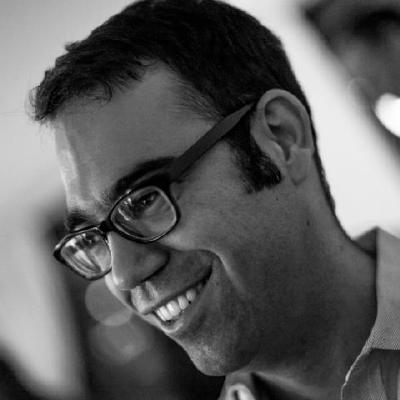
\includegraphics[height=10em]{figures/kyle.jpg}\\
        Kyle Cranmer\\
        {\scriptsize New York University}
      \end{column}
      \begin{column}[t]{0.45\textwidth}
          \centering
          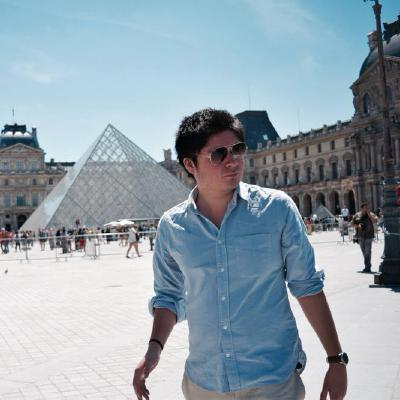
\includegraphics[height=10em]{figures/juan.jpg}\\
          Juan Pavez\\
          {\scriptsize Federico Santa Mar\'ia University}
      \end{column}
    \end{columns}

    \vspace{2em}

    See paper \citep{cranmer2015approximating} for full details.
\end{frame}

\begin{frame}
    \frametitle{Studying the constituents of the universe}

    \begin{columns}
        \begin{column}{0.55\textwidth}
            \centering
            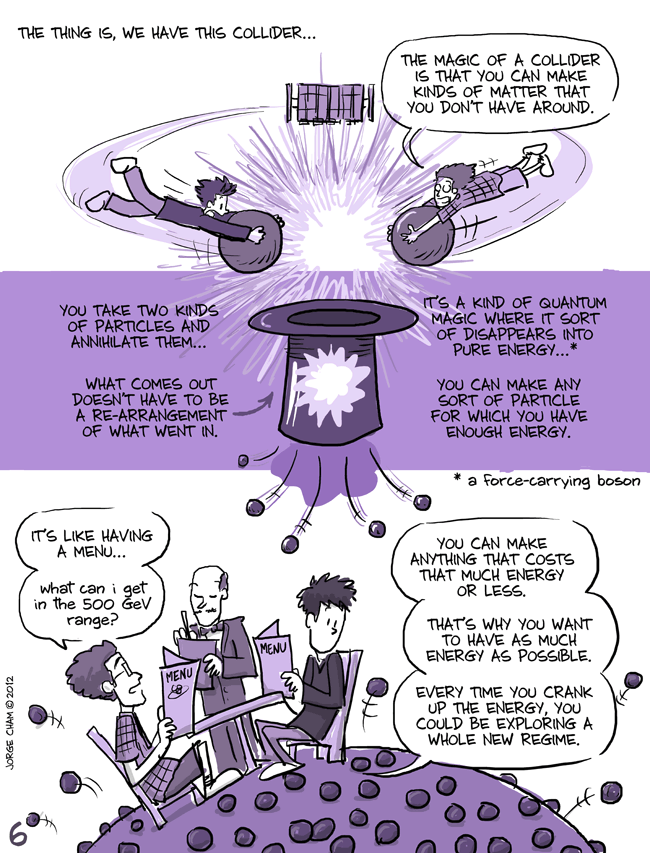
\includegraphics[width=\textwidth]{figures/phd1.png}\\
            {\scriptsize (c) Jorge Cham}
        \end{column}
        \begin{column}{0.4\textwidth}
            \centering
            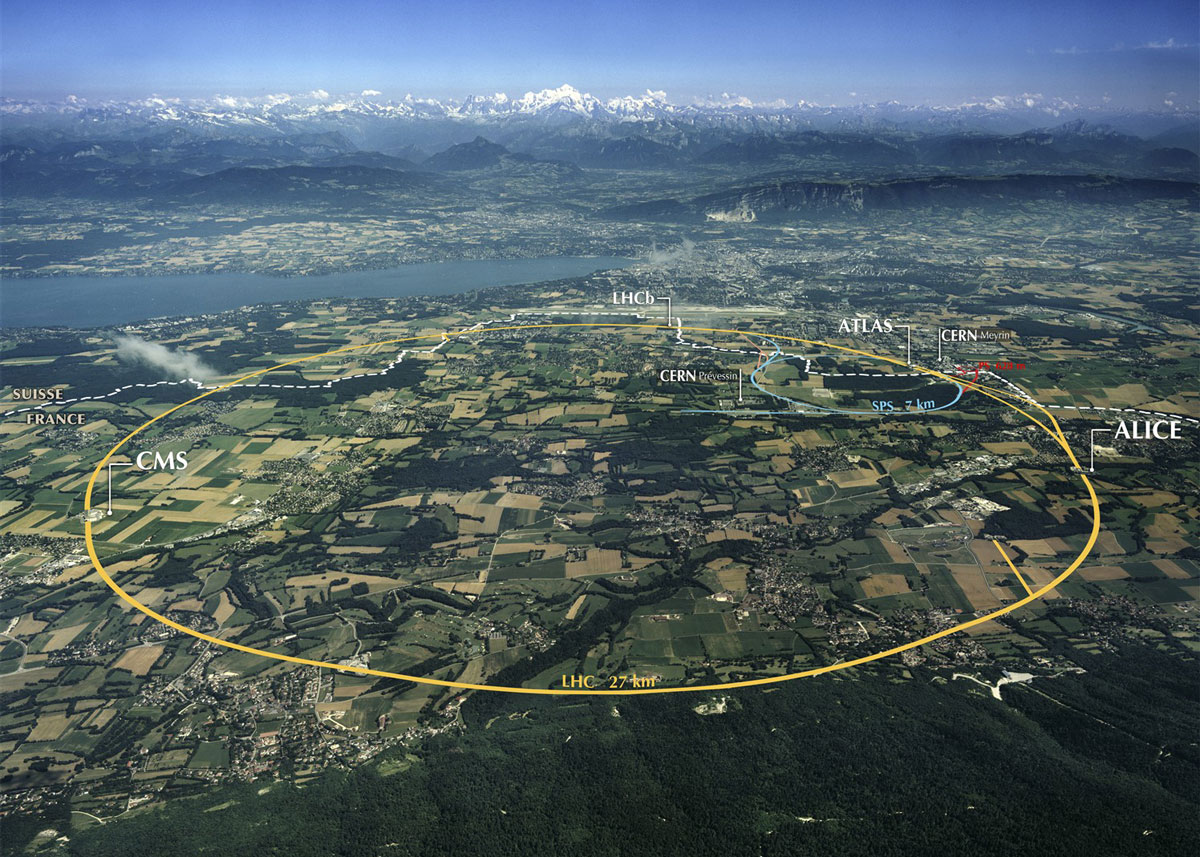
\includegraphics[width=\textwidth]{figures/lhc1.jpg}\\
            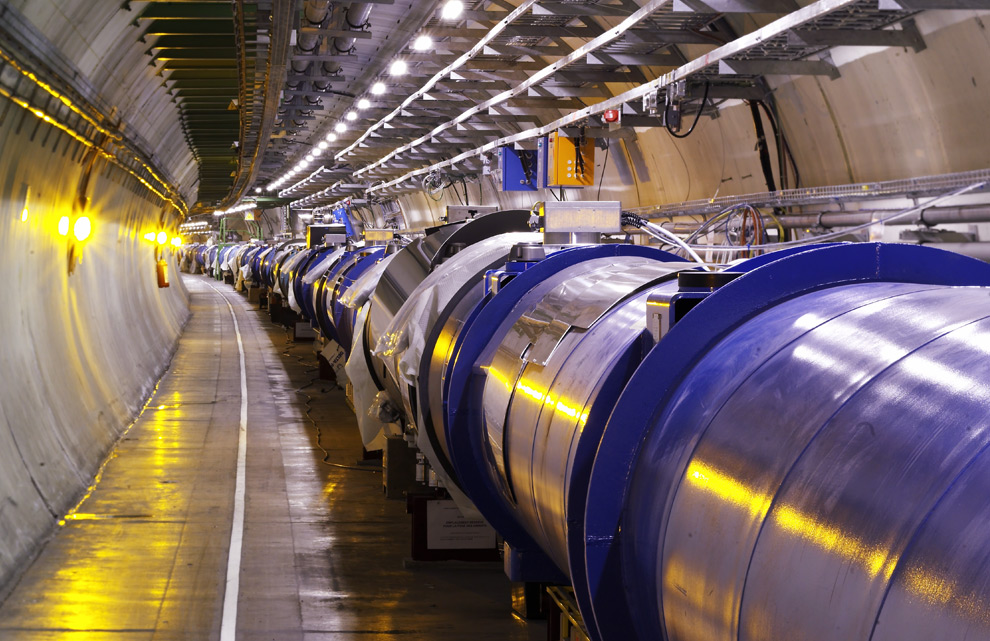
\includegraphics[width=\textwidth]{figures/lhc2.jpg}
        \end{column}
    \end{columns}


\end{frame}

\begin{frame}
    \frametitle{Collecting data}

    \begin{columns}
        \begin{column}{0.55\textwidth}
            \centering
            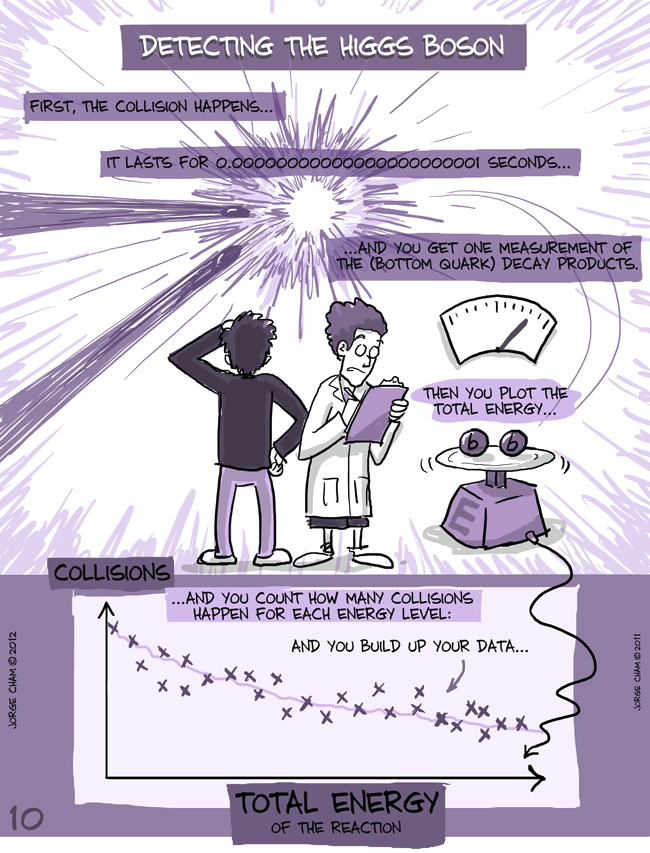
\includegraphics[width=\textwidth]{figures/phd2.png}\\
            {\scriptsize (c) Jorge Cham}
        \end{column}
        \begin{column}{0.4\textwidth}
            \centering
            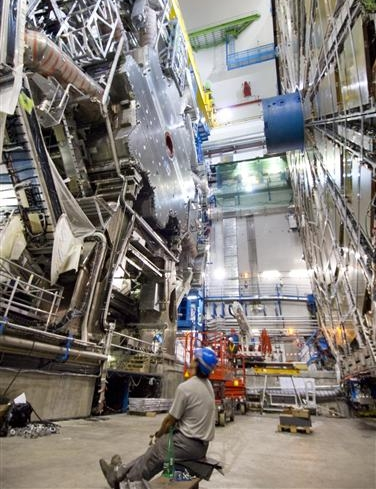
\includegraphics[width=\textwidth]{figures/lhc3.jpg}\\
            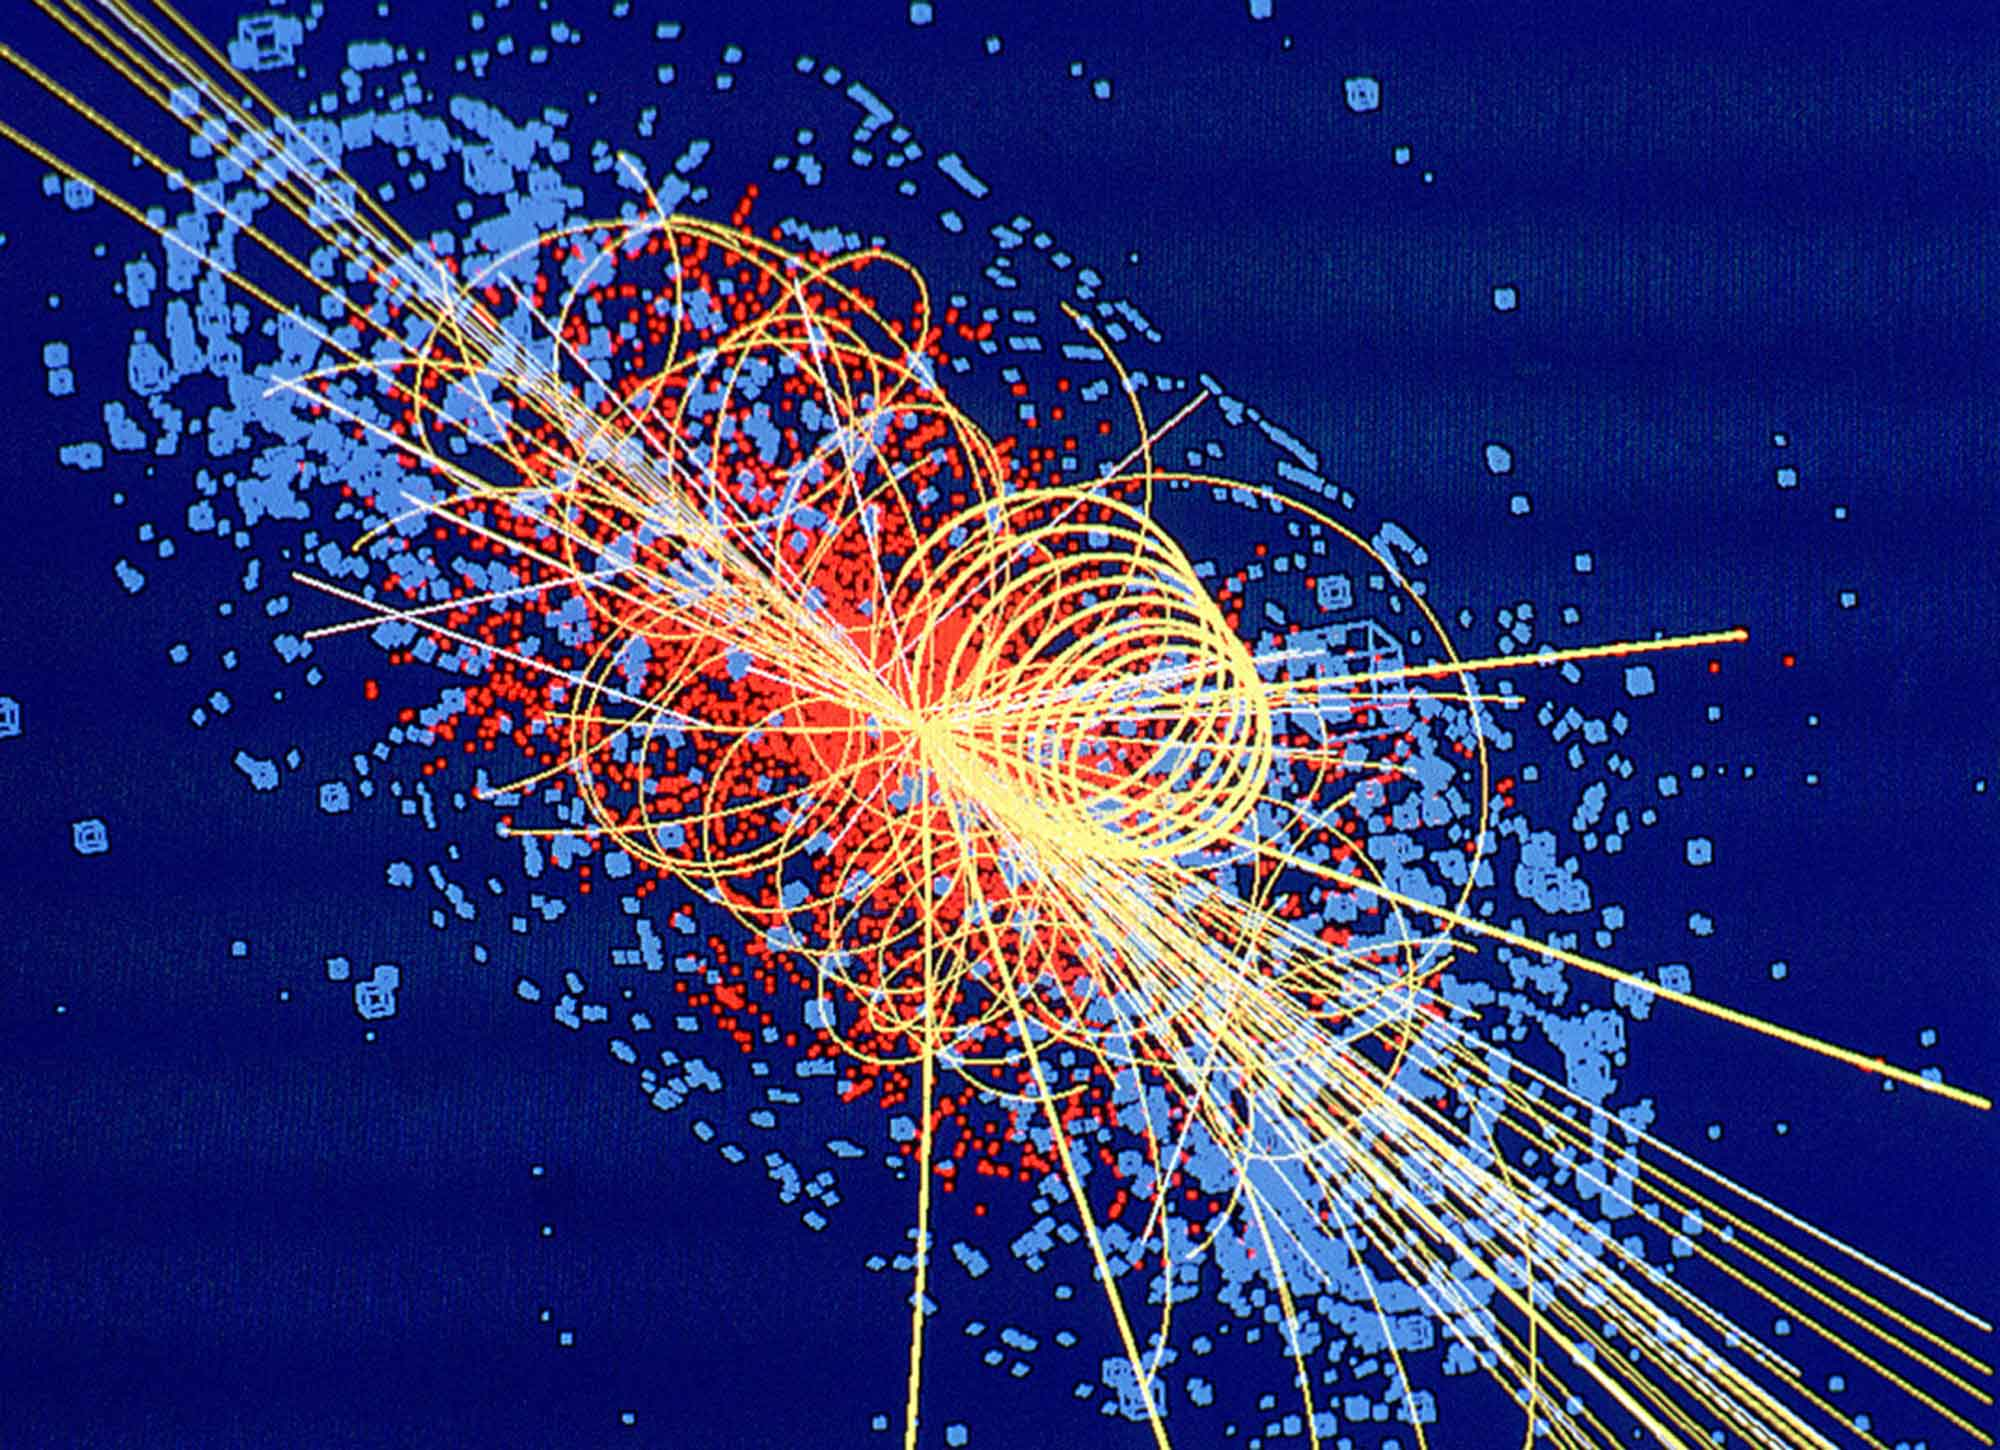
\includegraphics[width=\textwidth]{figures/lhc4.jpg}
        \end{column}
    \end{columns}
\end{frame}

\begin{frame}
    \frametitle{Testing for new physics}
    \vspace{0.5em}
    \begin{columns}
        \begin{column}{0.55\textwidth}
            \centering
            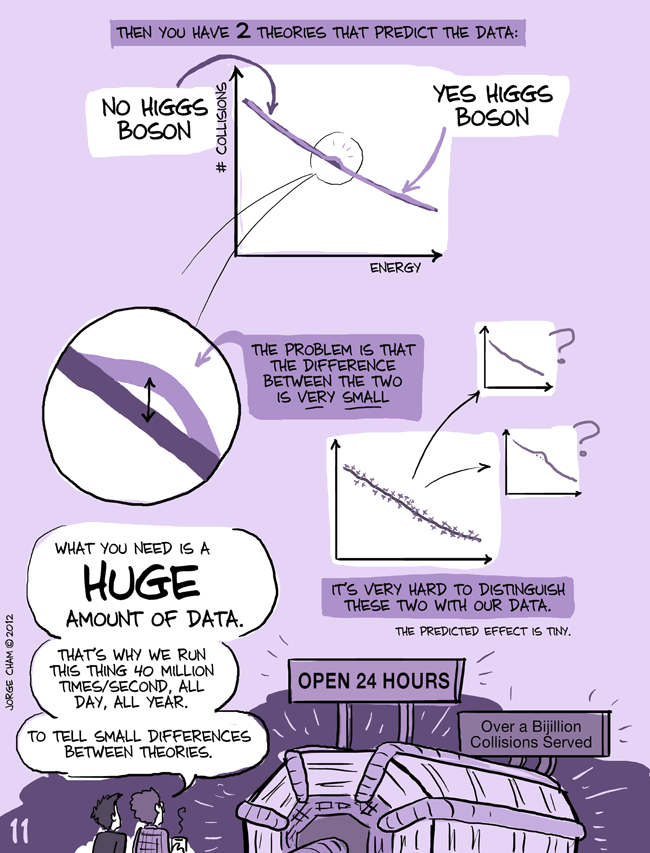
\includegraphics[width=\textwidth]{figures/phd3.png}\\
            {\scriptsize (c) Jorge Cham}
        \end{column}
        \begin{column}{0.4\textwidth}
            \centering
            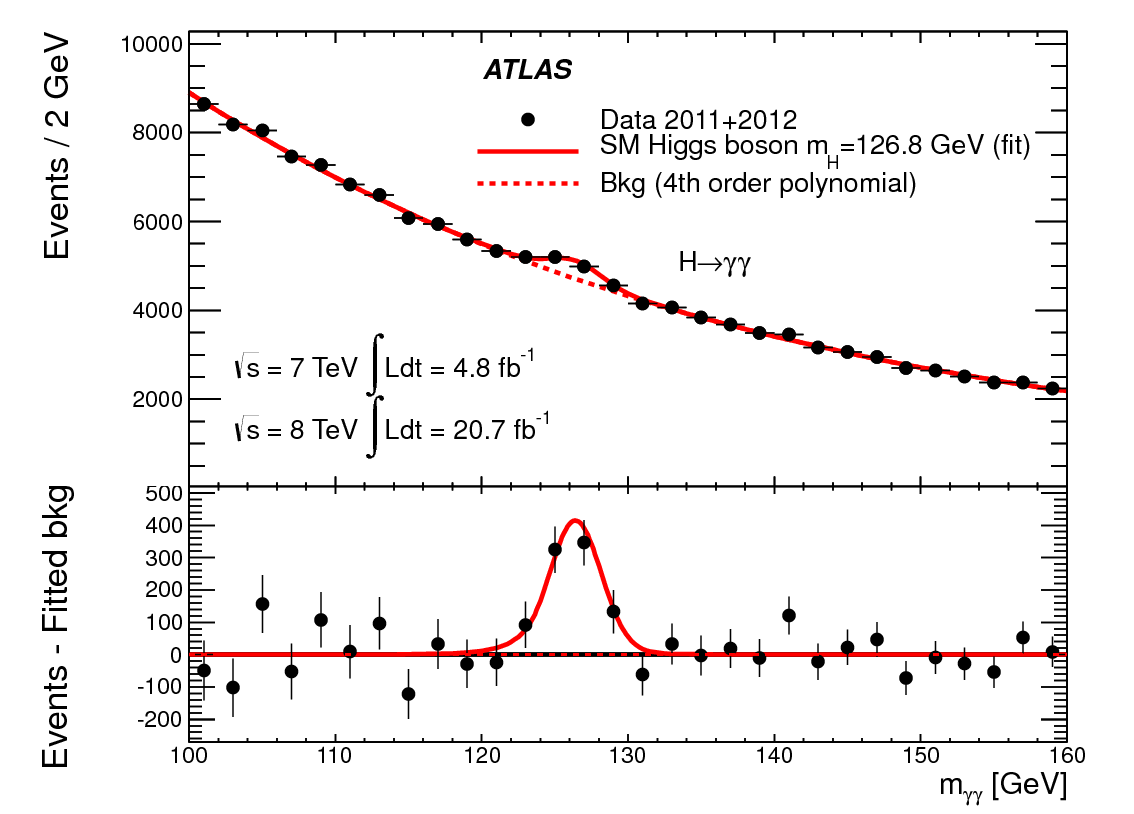
\includegraphics[width=\textwidth]{figures/plot-higgs.png}

            $$\frac{p(\text{data} | \text{theory} + X)}{p(\text{data} | \text{theory})}$$
        \end{column}
    \end{columns}
\end{frame}


\begin{frame}
    \frametitle{Likelihood-free setup}

    \begin{itemize}
        \item Complex simulator $p$ parameterized by $\theta$;
        \item Samples $\mathbf{x} \sim p$ can be generated on-demand;
        \item ... but the likelihood {\color{red} $p(\mathbf{x}|\theta)$ cannot be evaluated}!
    \end{itemize}

    \centering
    \begin{columns}
        \begin{column}{0.1\textwidth}
            \centering
            $p =$
        \end{column}
        \begin{column}{0.4\textwidth}
            \centering
            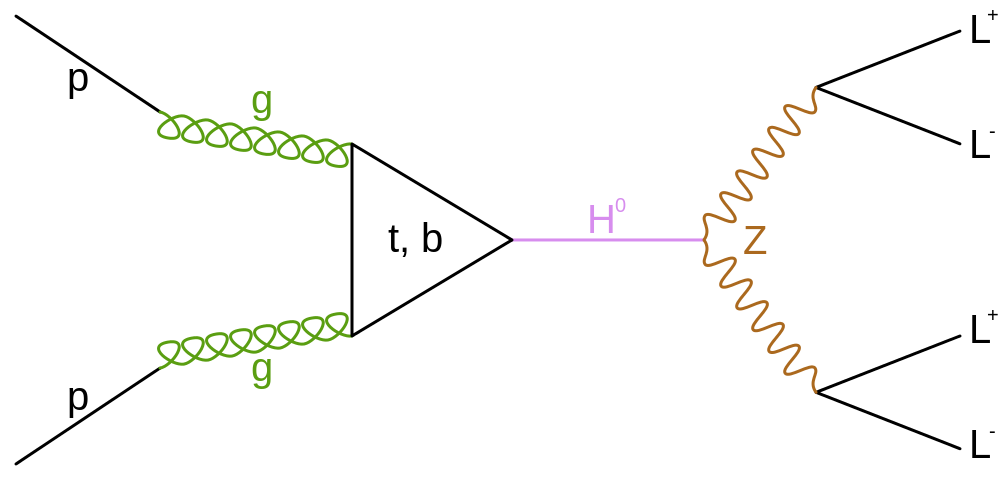
\includegraphics[width=\textwidth]{figures/feynman.png}
        \end{column}
        \begin{column}{0.1\textwidth}
            \centering
             $\otimes$
        \end{column}
        \begin{column}{0.4\textwidth}
            \centering
            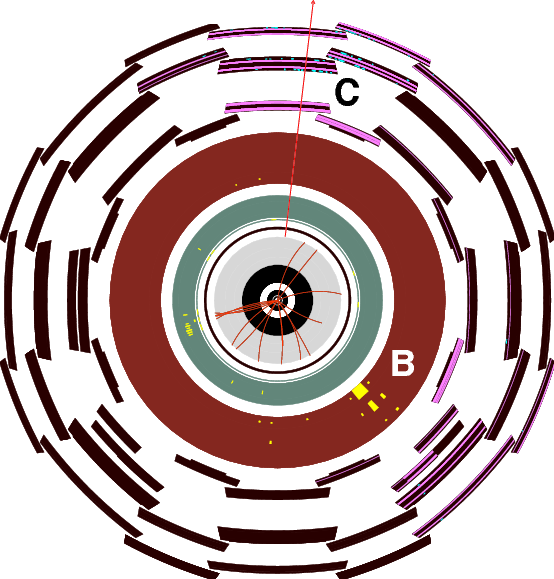
\includegraphics[width=\textwidth]{figures/atlas-sim.png}
        \end{column}
    \end{columns}

\end{frame}

\begin{frame}
    \frametitle{Simple hypothesis testing}

    \begin{itemize}
        \item Assume some observed data ${\cal D} = \{ \mathbf{x}_1, \dots, \mathbf{x}_n \}$;
        \item Test a null $\theta = \theta_0$ against an alternative $\theta = \theta_1$;
        \item The Neyman-Pearson lemma states that the most powerful test statistic is
            $$
            \lambda({\cal D}; \theta_0, \theta_1) = \prod_{\mathbf{x} \in {\cal D}} \frac{ p_\mathbf{X}(\mathbf{x}|\theta_0)}{ p_\mathbf{X}(\mathbf{x}|\theta_1)}.
            $$
        \item ... but neither $p_\mathbf{X}(\mathbf{x}|\theta_0)$ nor $p_\mathbf{X}(\mathbf{x}|\theta_1)$ can be evaluated!

    \end{itemize}

\end{frame}

\begin{frame}[fragile]
    \frametitle{Straight approximation}

    \begin{enumerate}
        \item Approximate $p_\mathbf{X}(\mathbf{x}|\theta_0)$ and $p_\mathbf{X}(\mathbf{x}|\theta_1)$ individually, using density estimation algorithms;
        \item Evaluate their ratio $r(\mathbf{x};\theta_0,\theta_1)$.
    \end{enumerate}

    \vspace{1em}

    Works fine for low-dimensional data, but because of the curse of dimensionality, this is in general a difficult problem! Moreover, {\color{red} it is not even necessary}!

    $$
      \mathnode{A}{  \frac{ p_\mathbf{X}(\mathbf{x}|\theta_0)}{ p_\mathbf{X}(\mathbf{x}|\theta_1)} } = \mathnode{B}{ r(\mathbf{x};\theta_0,\theta_1)}
    $$

    \begin{tikzpicture}[overlay]
      \path [>=stealth, ->, shorten <= 3pt, shorten >=3 pt, blue]
        (A) edge [bend left=60] (B);
      \path [>=stealth, ->, shorten <= 3pt, shorten >=3 pt, red]
        (B) edge [bend left=60] node {$/$} (A);
    \end{tikzpicture}

    \vspace{1em}

    {\small \centering \it When solving a problem of interest, do not solve a more general problem as an intermediate step. -- Vladimir Vapnik}

\end{frame}

\begin{frame}
    \frametitle{Likehood ratio invariance under change of variable}

    {\it Theorem.} The likelihood ratio is invariant under the change of variable $\mathbf{U} = s(\mathbf{X})$, provided $s(\mathbf{x})$ is monotonic with $r(\mathbf{x})$.

    $$
    r(\mathbf{x}) = \frac{ p_\mathbf{X}(\mathbf{x}|\theta_0)}{ p_\mathbf{X}(\mathbf{x}|\theta_1)} = \frac{ p_\mathbf{U}(s(\mathbf{x})|\theta_0)}{ p_\mathbf{U}(s(\mathbf{x})|\theta_1)}
    $$
\end{frame}

\begin{frame}
    \frametitle{Approximating likelihood ratios with classifiers}

    \begin{itemize}
        \item Well, a classifier trained to distinguish $\mathbf{x} \sim p_0$ from $\mathbf{x} \sim p_1$ approximates $$s^*(\mathbf{x}) = \frac{p_\mathbf{X}(\mathbf{x}|\theta_1)}{p_\mathbf{X}(\mathbf{x}|\theta_0) + p_\mathbf{X}(\mathbf{x}|\theta_1)},$$ which is monotonic with $r(\mathbf{x})$.

        \item Estimating $p(s(\mathbf{x})|\theta)$ is now easy, since the change of variable $s(\mathbf{x})$ projects $\mathbf{x}$ in a 1D space, where only the informative content of the ratio is preserved.

        \begin{itemize}
            \item This can be carried out using density estimation or calibration algorithms (histograms, KDE, isotonic regression, etc).
        \end{itemize}

        \item Disentangle training from calibration.
    \end{itemize}
\end{frame}

\begin{frame}
    \frametitle{Inference and composite hypothesis testing}

    Approximated likelihood ratios can be used for inference, since

    {\small
    \begin{align}\label{eqn:mle}
        \hat{\theta} &= \argmax_\theta  p({\cal D} | \theta) \nonumber \\
                     &= \argmax_\theta  \prod_{\mathbf{x} \in {\cal D}} \frac{p(\mathbf{x}| \theta)}{p(\mathbf{x}|\theta_1)} \nonumber \\
                     &= \argmax_\theta  \prod_{\mathbf{x} \in {\cal D}} \frac{p(s(\mathbf{x}; \theta, \theta_1) | \theta)}{p(s(\mathbf{x}; \theta, \theta_1) |\theta_1)} \;
    \end{align}}

    where $\theta_1$ is fixed and $s(\mathbf{x}; \theta, \theta_1)$ is a family of classifiers parameterized by $(\theta, \theta_1)$.

    \vspace{1em}

    Accordingly, generalized (or profile) likelihood ratio tests can be evaluated in the same way.
\end{frame}

\begin{frame}
    \frametitle{Parameterized learning}

    For inference, we need to build a family $s(\mathbf{x}; \theta, \theta_1)$ of classifiers.

    \begin{itemize}
        \item One could build a classifier $s$ independently for all $\theta, \theta_1$. But this is computationally expensive and would not guarantee a smooth evolution of $s(\mathbf{x}; \theta, \theta_1)$ as $\theta$ varies.

        \item Solution: build a single parameterized classifier instead, where parameters are additional input features~\citep{cranmer2015approximating,Baldi:2016fzo}.

    \end{itemize}

    \begin{columns}
      \begin{column}[b]{0.48\textwidth}
          {\scriptsize
          \begin{algorithmic}
              \State ${\cal T := \{ \}}$;
              \While{ $\text{size}({\cal T}) < N $ }
                  %\State Select or draw $\theta_0$, $\theta_1$ from $\Theta_0$, $\Theta_1$;
                  \State Draw $\theta_0 \sim \pi_{\Theta_0}$;
          	    \State Draw $\mathbf{x} \sim p(\mathbf{x}|\theta_0)$;
          		\State ${\cal T} := {\cal T} \cup \{ ((\mathbf{x}, \theta_0, \theta_1), y=0) \}$;
                  \State Draw $\theta_1 \sim \pi_{\Theta_1}$;
          		\State Draw $\mathbf{x} \sim p(\mathbf{x}|\theta_1)$;
          		\State ${\cal T} := {\cal T} \cup \{ ((\mathbf{x}, \theta_0, \theta_1), y=1) \}$;
              \EndWhile
              \State Learn a single classifier $s(\mathbf{x}; \theta_0, \theta_1)$ from ${\cal T}$.
          \end{algorithmic}}
      \end{column}
      \begin{column}[b]{0.48\textwidth}
          \centering
          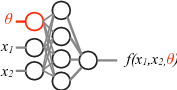
\includegraphics[width=0.5\textwidth]{figures/networks.png}
          \vspace{1cm}
      \end{column}
    \end{columns}





\end{frame}

\begin{frame}
    \frametitle{Example: Inference from multidimensional data}

\begin{columns}
    \begin{column}{0.55\textwidth}
       Let assume 5D data $\mathbf{x}$ generated
       from the following process $p_0$:

            {\scriptsize
           \begin{enumerate}
               \item $\mathbf{z} := (z_0, z_1, z_2, z_3, z_4)$, such that
                   $z_0 \sim {\cal N}(\mu=\alpha, \sigma=1)$,
                   $z_1 \sim {\cal N}(\mu=\beta, \sigma=3)$,
                   $z_2 \sim {\text{Mixture}}(\frac{1}{2}\,{\cal N}(\mu=-2, \sigma=1), \frac{1}{2}\,{\cal N}(\mu=2, \sigma=0.5))$,
                   $z_3 \sim {\text{Exponential}(\lambda=3)}$, and
                   $z_4 \sim {\text{Exponential}(\lambda=0.5)}$;
               \item $\mathbf{x} := R  \mathbf{z}$, where $R$ is a fixed
               semi-positive definite $5 \times 5$ matrix defining a fixed projection
               of $\mathbf{z}$ into the observed space.
           \end{enumerate}}

        Our goal is to infer the values $\alpha$ and $\beta$ based on ${\cal D}$.
    \end{column}
    \begin{column}{0.4\textwidth}
        \centering
        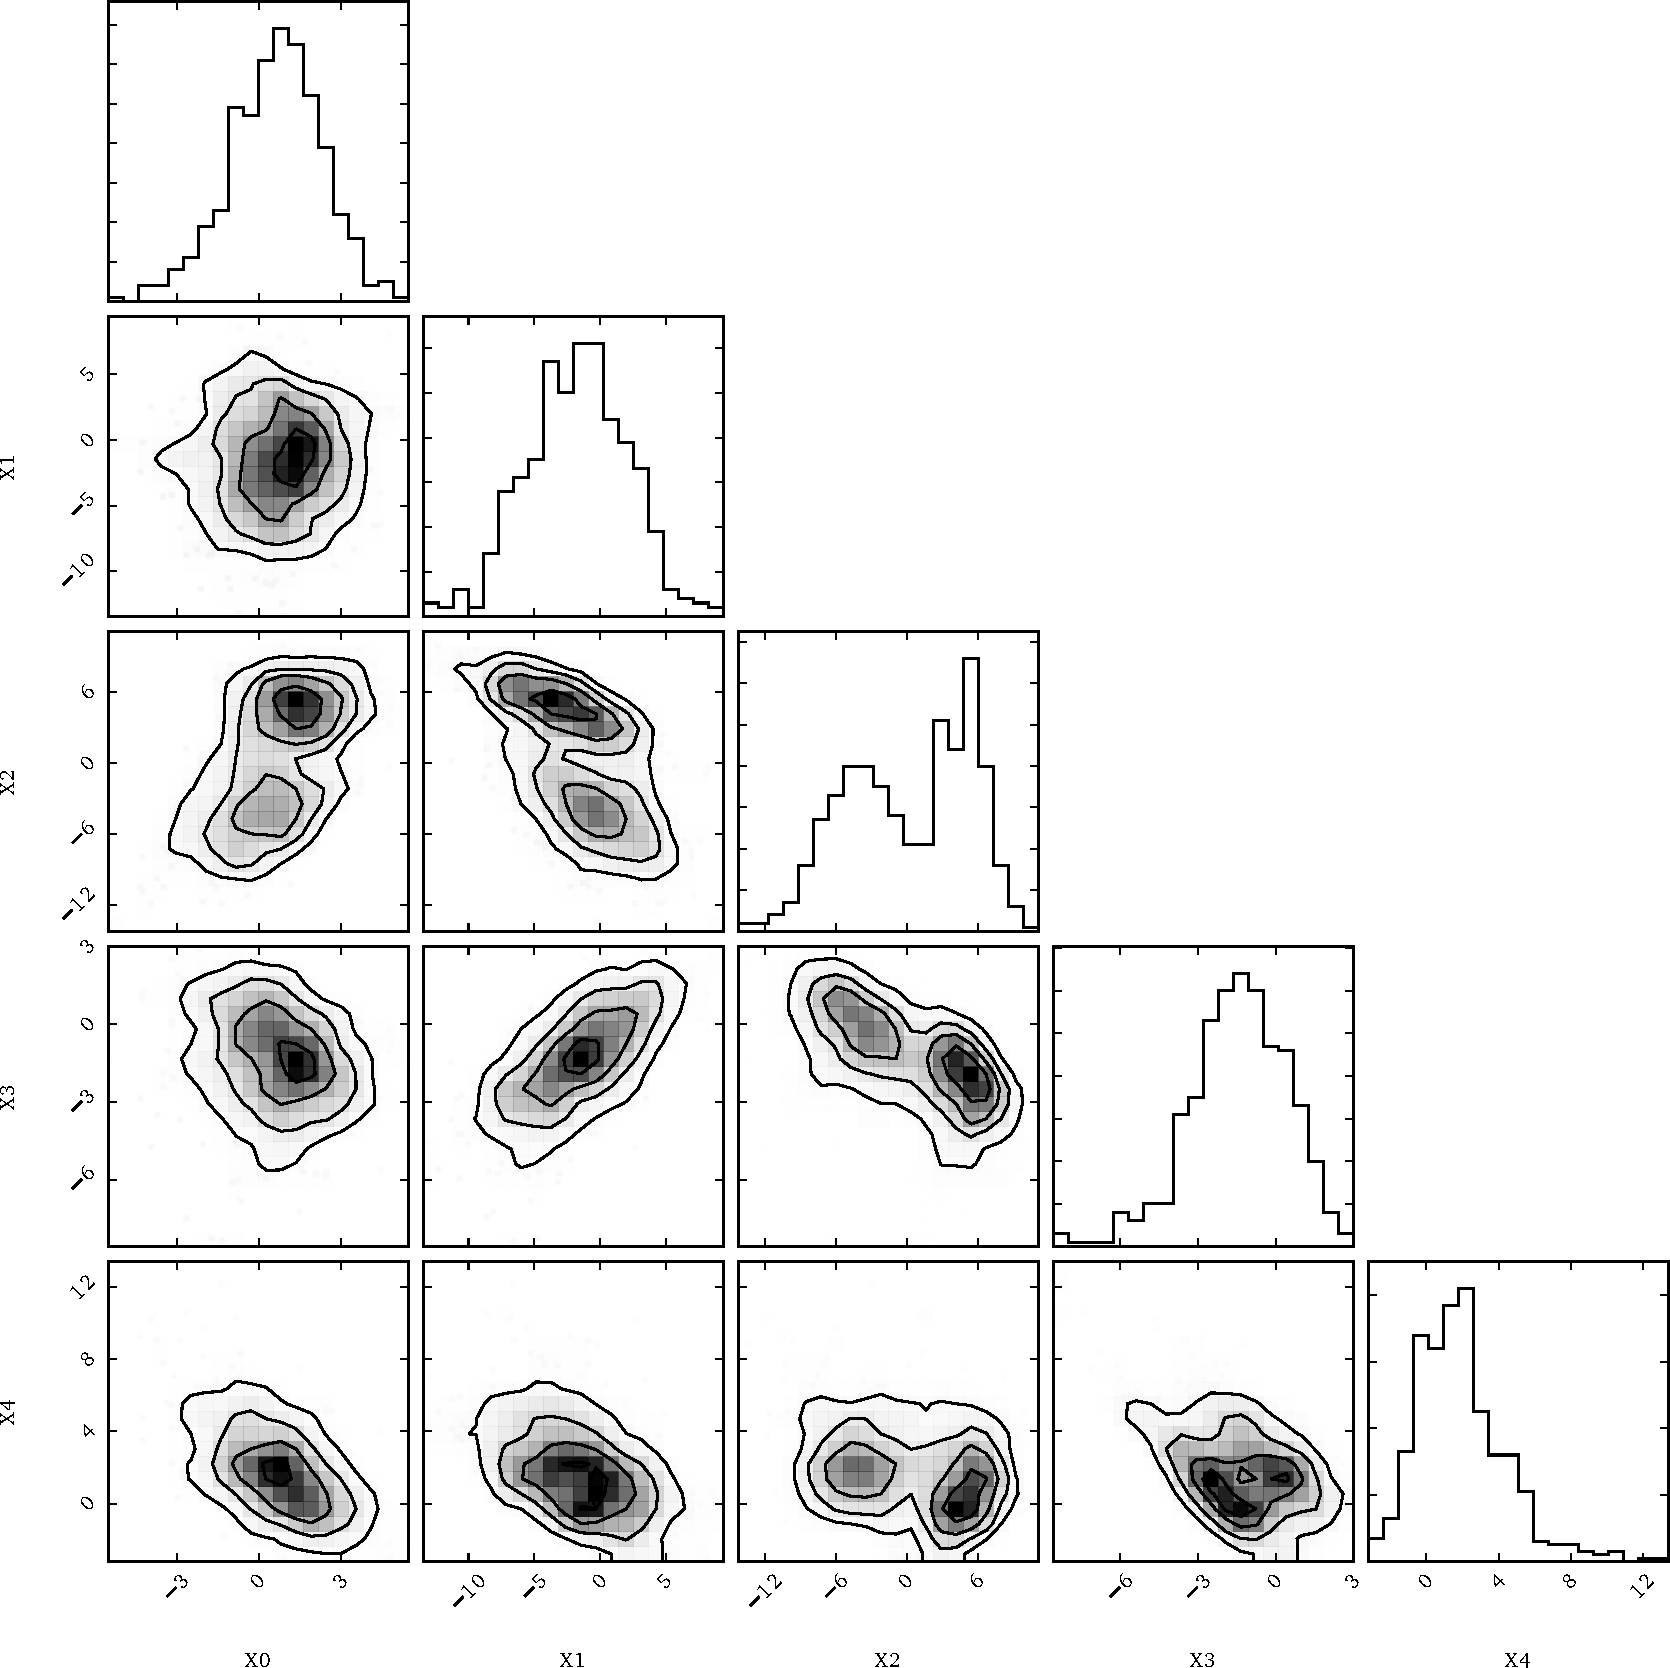
\includegraphics[width=\textwidth]{figures/fig4.pdf}\\
        Observed data ${\cal D}$
    \end{column}
\end{columns}

\vspace{2em}

\centering

\includegraphics[height=0.8em]{figures/github.png}~ {\it \small Check out \citep{carl} to reproduce this example.}
\vspace{-1em}

\end{frame}

\begin{frame}
    \frametitle{Example: Inference from multidimensional data}

    Recipe:

    \begin{enumerate}
        \item Build a single parameterized classifier $s(\mathbf{x}; \theta_0, \theta_1)$,
        in this case a 2-layer NN trained on 5+2 features, with the alternative fixed to $\theta_1=(\alpha=0, \beta=0)$.

        \item Find the approximated MLE $\hat \alpha, \hat \beta$ by solving Eqn.~\ref{eqn:mle}.
            \begin{itemize}
                \item Solve Eqn.~\ref{eqn:mle} using likelihood scans or through optimization.
                \item Since the generator is inexpensive, $p(s(\mathbf{x}; \theta_0, \theta_1)|\theta)$ can be calibrated on-the-fly, for every candidate $(\alpha,\beta)$, e.g. using histograms.
            \end{itemize}

        \item Construct the log-likelihood ratio (LLR) statistic
        \begin{equation*}
            -2 \log \Lambda(\alpha, \beta ) = -2 \log \frac{p({\cal D} | \alpha, \beta)}{  p({\cal D} | \hat \alpha, \hat \beta) }
        \end{equation*}

    \end{enumerate}

\end{frame}

\begin{frame}


    \begin{columns}
      \begin{column}[b]{0.48\textwidth}
        \centering
        \small Exact $-2 \log \Lambda(\alpha, \beta )$\\
        \vspace{0.5em}
        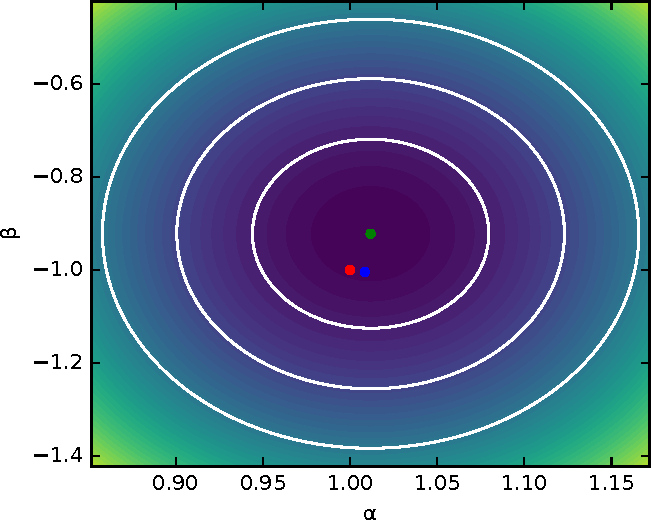
\includegraphics[height=10em]{figures/fig5a.pdf}
      \end{column}
      \begin{column}[b]{0.48\textwidth}
          \centering
          \small Approx. LLR (smoothed by a Gaussian Process)\\
          \vspace{0.5em}
          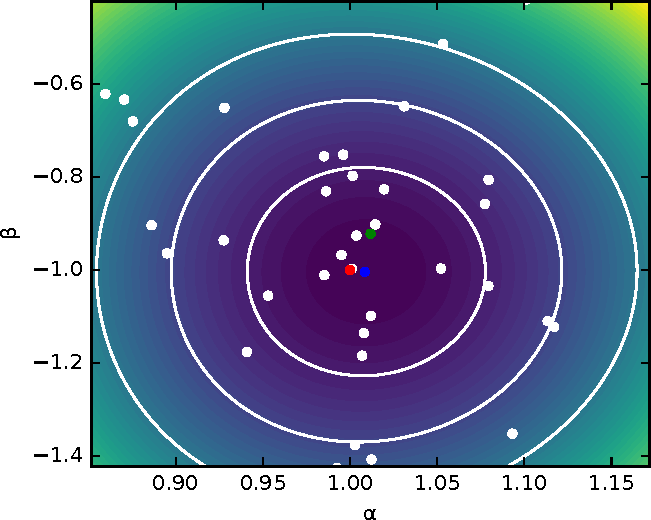
\includegraphics[height=10em]{figures/fig5c.pdf}
      \end{column}
    \end{columns}

    \vspace{1em}

    \centering
    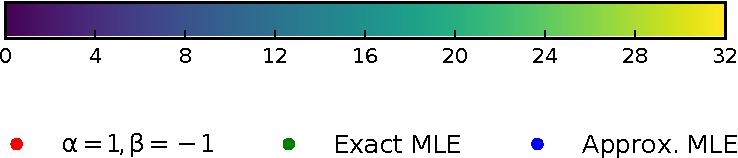
\includegraphics[width=0.5\textwidth]{figures/fig5d.pdf}

\end{frame}

\begin{frame}
    \frametitle{Diagnostics}

    In practice $\hat{r}(\hat{s}(\mathbf{x}; \theta_0, \theta_1))$ will not be exact.  Diagnostic procedures are needed to assess the quality of this approximation.

    \begin{enumerate}
        \item For inference, the value of the MLE $\hat{\theta}$ should be independent of the value of $\theta_1$ used in the denominator of the ratio.
        \item Train a classifier to distinguish between unweighted samples from $p(\mathbf{x}|\theta_0)$ and samples from $p(\mathbf{x}|\theta_1)$ weighted by $\hat{r}(\hat{s}(\mathbf{x}; \theta_0, \theta_1))$.
    \end{enumerate}

    \vspace{-2em}

    \begin{center}
            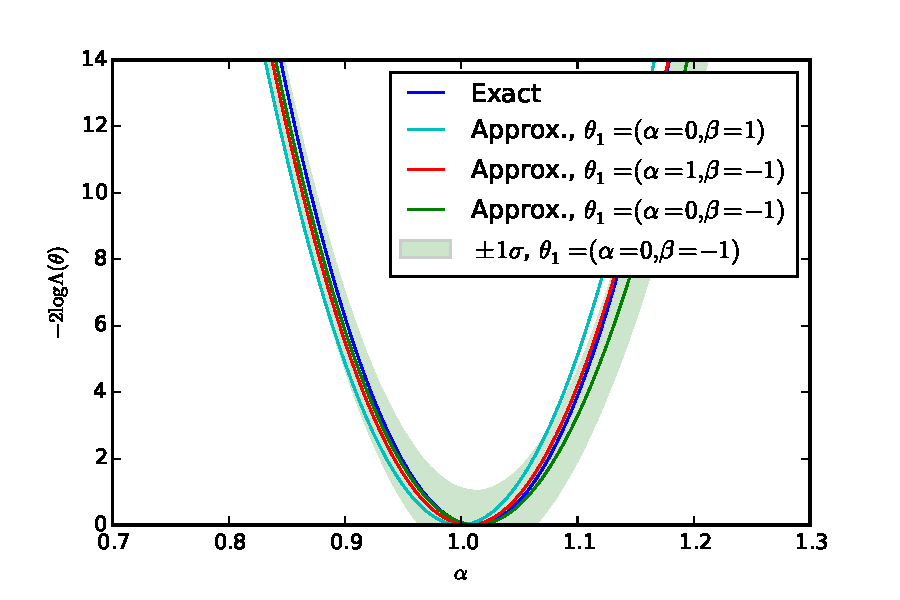
\includegraphics[clip, trim=0.3cm 0.3cm 0.3cm 0.3cm,height=10.075em]{figures/likelihood_comp_2.pdf}
            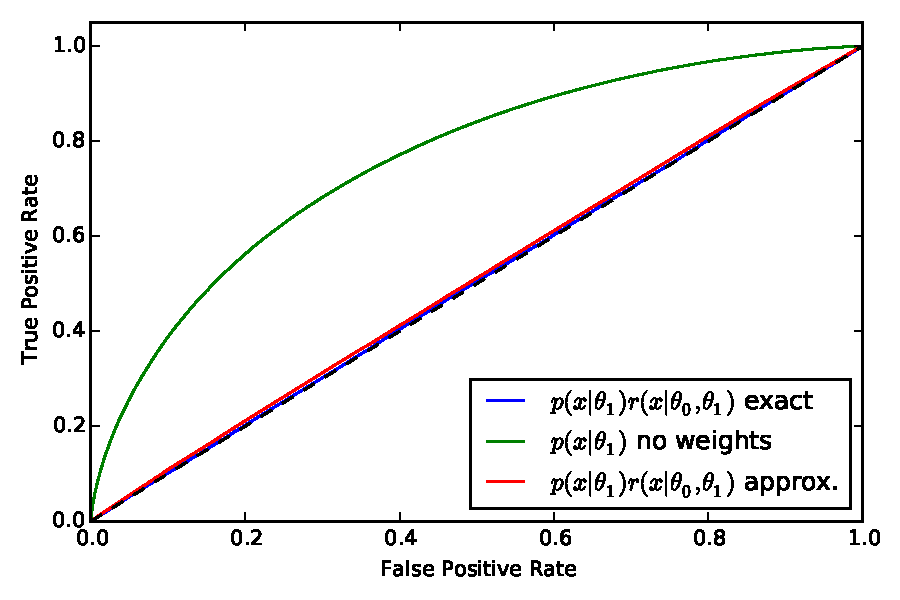
\includegraphics[clip, trim=0.3cm 0.3cm 0.3cm 0.3cm,height=9.5em]{figures/ROC_comp2.pdf}
    \end{center}

\end{frame}

\begin{frame}
    \frametitle{Density ratio estimation}

    The density ratio $r(\mathbf{x} ; \theta_0, \theta_1) = \frac{p(\mathbf{x}|\theta_0)} { p(\mathbf{x}|\theta_1) }$ appears in many other fundamental statistical inference problems, including

    \begin{itemize}
        \item transfer learning,
        \item outlier detection,
        \item divergence estimation,
        \item ...
    \end{itemize}

    {\color{red} For all of them, the proposed approximation can be used as a drop-in replacement!}
\end{frame}

\begin{frame}
    \frametitle{Transfer learning}

    Under the assumption that train and test data are drawn iid from a same distribution $p$,
    $$\frac{1}{N} \sum_{\mathbf{x}_i} L(\varphi(\mathbf{x}_i)) \to \int L(\varphi(\mathbf{x})) {\color{red} p(\mathbf{x})} d\mathbf{x},$$
    as training data increases, i.e. as $N \to \infty$.

    \vspace{1cm}

    Minimizing $L$ over training data is therefore a {\color{blue} good strategy}.


\end{frame}

\begin{frame}
    \frametitle{Transfer learning}

    \sout{Under the assumption that train and test data are drawn iid from a same distribution $p$,}
    $$\frac{1}{N} \sum_{\mathbf{x}_i} L(\varphi(\mathbf{x}_i)) \to \int L(\varphi(\mathbf{x})) {\color{red} p_\text{train}(\mathbf{x})} d\mathbf{x},$$
    as training data increases, i.e. as $N \to \infty$.

    \vspace{1cm}

    But we want to be good on test data, i.e., minimize
    $$\int L(\varphi(\mathbf{x})) {\color{blue} p_\text{test}(\mathbf{x})} d\mathbf{x}.$$

    Minimizing $L$ over training data is therefore a {\color{red} bad strategy}!

\end{frame}

\begin{frame}
    \frametitle{Importance weighting}

    Reweight samples by $\frac{\color{blue} p_\text{test}(\mathbf{x}_i)}{\color{red} p_\text{train}(\mathbf{x}_i)}$, such that

    $$\frac{1}{N} \sum_{\mathbf{x}_i} \frac{\color{blue} p_\text{test}(\mathbf{x}_i)}{\color{red} p_\text{train}(\mathbf{x}_i)}  L(\varphi(\mathbf{x}_i)) \to \int \frac{\color{blue}  p_\text{test}(\mathbf{x})}{\color{red} p_\text{train}(\mathbf{x})} L(\varphi(\mathbf{x})) {\color{red} p_\text{train}(\mathbf{x})}  d\mathbf{x},$$
    as training data increases, i.e. as $N \to \infty$.

    \vspace{1cm}

    Again, $\frac{\color{blue} p_\text{test}(\mathbf{x}_i)}{\color{red} p_\text{train}(\mathbf{x}_i)}$ cannot be evaluated directly, but approximated likelihood ratios can be used as a drop-in replacement.
\end{frame}

\begin{frame}
    \frametitle{Example}

    $p_0 : \alpha=-2, \beta=2$ \textit{versus}
    $p_1 : \alpha=0, \beta=0$
    \begin{center}
        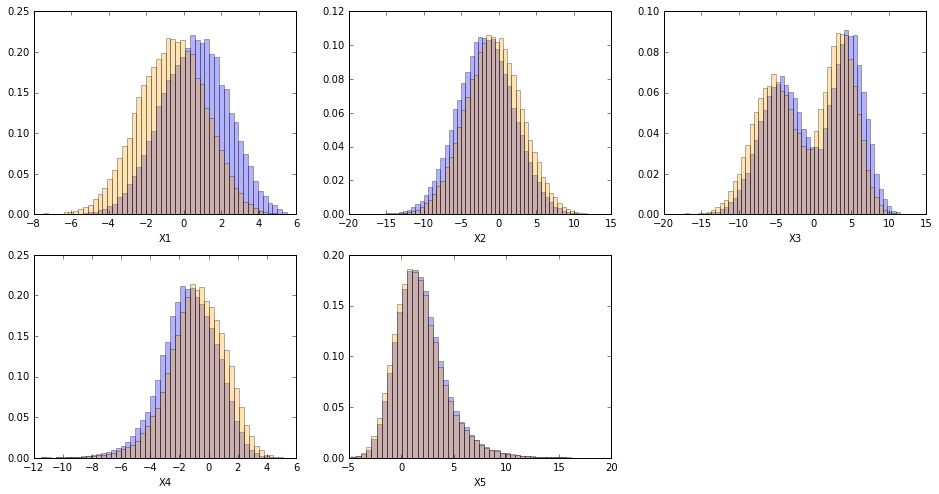
\includegraphics[width=0.6\textwidth]{figures/reweight1.png}
    \end{center}

    $p_0$  \textit{versus} $\frac{p_0}{p_1} p_1$
    \begin{center}
        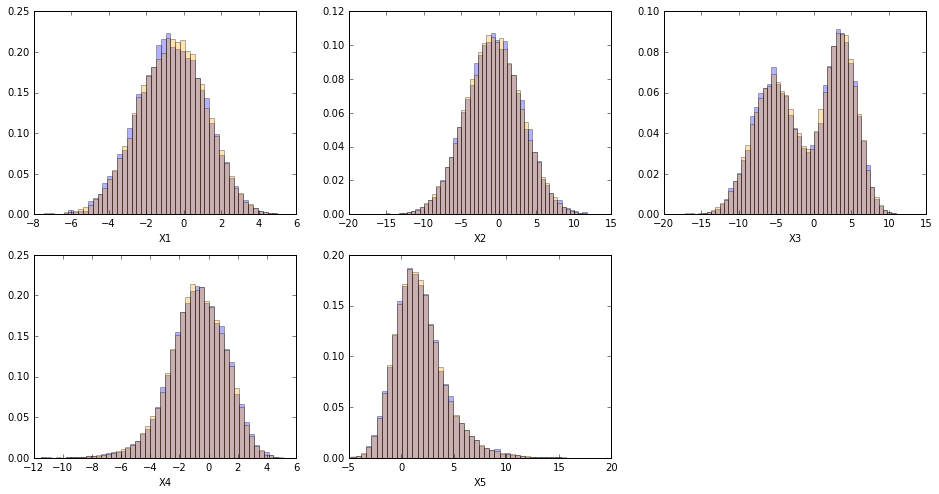
\includegraphics[width=0.6\textwidth]{figures/reweight2.png}
    \end{center}
\end{frame}

\begin{frame}
    \frametitle{Example}

    $p_0$  \textit{versus} $\hat{r} p_1$
    \begin{center}
        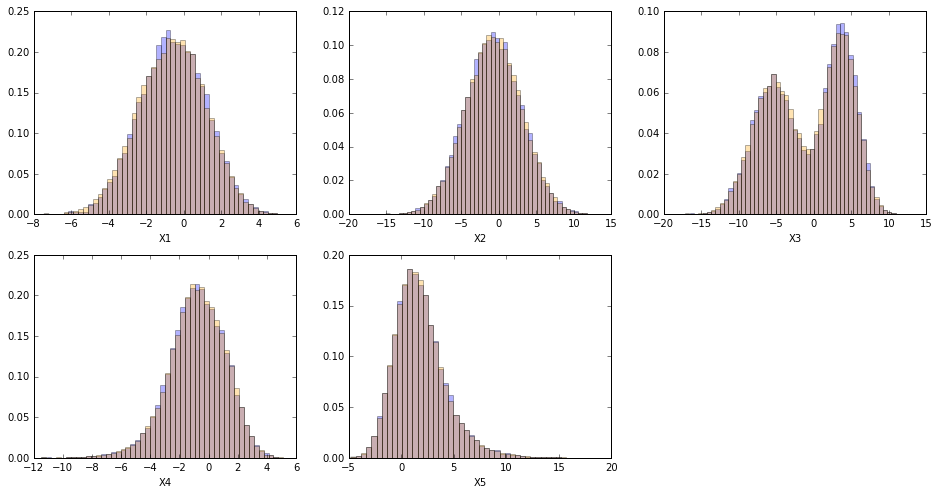
\includegraphics[width=0.6\textwidth]{figures/reweight3.png}
    \end{center}

    \begin{center}
        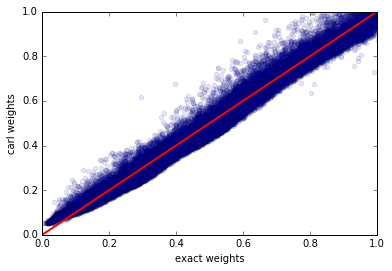
\includegraphics[width=0.4\textwidth]{figures/reweight4.png}
    \end{center}
\end{frame}

\begin{frame}
    \frametitle{Summary}

    \begin{itemize}
        \item We proposed an approach for approximating LR in the likelihood-free setup.

        \item Evaluating likelihood ratios reduces to supervised learning. Both problems are deeply connected.

        \item Alternative to Approximate Bayesian Computation, without the need to define a prior over parameters.
    \end{itemize}
\end{frame}

\begin{frame}[plain,noframenumbering]
    \frametitle{References}
    {\footnotesize
    \bibliographystyle{apalike}
    \bibliography{biblio}}
\end{frame}


\end{document}
